\section{Программная реализация задачи}

\href{https://github.com/utpwtb/ITMO/tree/main/4%20%D0%92%D1%8B%D1%87%D0%B8%D1%81%D0%BB%D0%B8%D1%82%D0%B5%D0%BB%D1%8C%D0%BD%D0%B0%D1%8F%20%D0%9C%D0%B0%D1%82%D0%B5%D0%BC%D0%B0%D1%82%D0%B8%D0%BA%D0%B0/%D0%9F%D1%80%D0%BE%D0%B3%D1%80%D0%B0%D0%BC%D0%BC%D0%B0/Lab4/CM_Lab4}{{\color{blue} GitHub - Лабораторная работа №4}}

\subsection{Метод наименьших квадратов (LSMSolver.java)}

\begin{lstlisting}[style=javaStyle, label=code:lsm]
public class LSMSolver {

    private static void computeQuality(ApproximationResult result, List<Double> x, List<Double> y,
                                       Function<Double, Double> phi) {
        int n = x.size();
        double meanY = y.stream().mapToDouble(Double::doubleValue).average().orElse(0);

        double[] yPred = new double[n];
        double[] res = new double[n];

        double ssRes = 0, ssTot = 0;
        for (int i = 0; i < n; i++) {
            double yi = y.get(i);
            double pi = phi.apply(x.get(i));
            yPred[i] = pi;
            double eps = pi - yi;
            res[i] = eps;
            ssRes += eps * eps;
            ssTot += (yi - meanY) * (yi - meanY);
        }

        result.setS(ssRes);
        result.setDelta(Math.sqrt(ssRes / n));
        result.setYPredicted(yPred);
        result.setResiduals(res);

        double r2 = ssTot == 0 ? 1.0 : 1 - ssRes / ssTot;
        result.setR2(r2);

        double meanX = x.stream().mapToDouble(Double::doubleValue).average().orElse(0);
        double cov = 0, varX = 0, varY = 0;
        for (int i = 0; i < n; i++) {
            cov += (x.get(i) - meanX) * (y.get(i) - meanY);
            varX += (x.get(i) - meanX) * (x.get(i) - meanX);
            varY += (y.get(i) - meanY) * (y.get(i) - meanY);
        }
        double denom = Math.sqrt(varX * varY);
        result.setPearsonR(denom == 0 ? 0 : cov / denom);
    }

    public static ApproximationResult linear(List<Double> x, List<Double> y) {
        int n = x.size();
        double sX = 0, sXX = 0, sY = 0, sXY = 0;
        for (int i = 0; i < n; i++) {
            double xi = x.get(i), yi = y.get(i);
            sX += xi; sXX += xi * xi; sY += yi; sXY += xi * yi;
        }
        double det = sXX * n - sX * sX;
        double a = (sXY * n - sX * sY) / det;
        double b = (sXX * sY - sX * sXY) / det;

        ApproximationResult result = new ApproximationResult("Линейная функция", new double[]{a, b});
        computeQuality(result, x, y, xi -> a * xi + b);
        return result;
    }

    public static ApproximationResult quadratic(List<Double> x, List<Double> y) {
        int n = x.size();
        double sX = 0, sX2 = 0, sX3 = 0, sX4 = 0, sY = 0, sXY = 0, sX2Y = 0;
        for (int i = 0; i < n; i++) {
            double xi = x.get(i), yi = y.get(i);
            double x2 = xi * xi;
            sX += xi; sX2 += x2; sX3 += x2 * xi; sX4 += x2 * x2;
            sY += yi; sXY += xi * yi; sX2Y += x2 * yi;
        }
        double[][] A = {{n, sX, sX2}, {sX, sX2, sX3}, {sX2, sX3, sX4}};
        double[] B = {sY, sXY, sX2Y};
        double[] coeffs = solveGauss(A, B, 3);

        ApproximationResult result = new ApproximationResult("Квадратичный полином", coeffs);
        computeQuality(result, x, y, xi -> coeffs[0] + coeffs[1] * xi + coeffs[2] * xi * xi);
        return result;
    }

    public static ApproximationResult cubic(List<Double> x, List<Double> y) {
        int n = x.size();
        double sX = 0, sX2 = 0, sX3 = 0, sX4 = 0, sX5 = 0, sX6 = 0;
        double sY = 0, sXY = 0, sX2Y = 0, sX3Y = 0;
        for (int i = 0; i < n; i++) {
            double xi = x.get(i), yi = y.get(i);
            double x2 = xi * xi, x3 = x2 * xi;
            sX += xi; sX2 += x2; sX3 += x3; sX4 += x2 * x2;
            sX5 += x3 * x2; sX6 += x3 * x3;
            sY += yi; sXY += xi * yi; sX2Y += x2 * yi; sX3Y += x3 * yi;
        }
        double[][] A = {
                {n, sX, sX2, sX3},
                {sX, sX2, sX3, sX4},
                {sX2, sX3, sX4, sX5},
                {sX3, sX4, sX5, sX6}
        };
        double[] B = {sY, sXY, sX2Y, sX3Y};
        double[] coeffs = solveGauss(A, B, 4);

        ApproximationResult result = new ApproximationResult("Кубический полином", coeffs);
        computeQuality(result, x, y, xi -> coeffs[0] + coeffs[1] * xi + coeffs[2] * xi * xi + coeffs[3] * xi * xi * xi);
        return result;
    }

    public static ApproximationResult exponential(List<Double> x, List<Double> y) {
        List<Double> lnY = y.stream().map(v -> {
            if (v <= 0) return Double.NaN;
            return Math.log(v);
        }).collect(Collectors.toList());

        if (lnY.contains(Double.NaN)) {
            ApproximationResult bad = new ApproximationResult("Экспоненциальная функция", new double[]{0, 0});
            bad.setS(Double.MAX_VALUE);
            bad.setDelta(Double.MAX_VALUE);
            bad.setR2(0);
            bad.setR2Message("Данные содержат неположительные значения, экспоненциальная аппроксимация невозможна");
            bad.setYPredicted(new double[x.size()]);
            bad.setResiduals(new double[x.size()]);
            return bad;
        }

        ApproximationResult lin = linear(x, lnY);
        // ln(y) = A·x + B, 其中 A = b, B = ln(a) → a = exp(B), b = A
        double a = Math.exp(lin.getCoefficients()[1]);
        double b = lin.getCoefficients()[0];

        ApproximationResult result = new ApproximationResult("Экспоненциальная функция", new double[]{a, b});
        computeQuality(result, x, y, xi -> a * Math.exp(b * xi));
        return result;
    }

    public static ApproximationResult logarithmic(List<Double> x, List<Double> y) {
        List<Double> lnX = x.stream().map(v -> {
            if (v <= 0) return Double.NaN;
            return Math.log(v);
        }).collect(Collectors.toList());

        if (lnX.contains(Double.NaN)) {
            ApproximationResult bad = new ApproximationResult("Логарифмическая функция", new double[]{0, 0});
            bad.setS(Double.MAX_VALUE);
            bad.setDelta(Double.MAX_VALUE);
            bad.setR2(0);
            bad.setR2Message("Данные содержат неположительные значения, логарифмическая аппроксимация невозможна");
            bad.setYPredicted(new double[x.size()]);
            bad.setResiduals(new double[x.size()]);
            return bad;
        }

        ApproximationResult lin = linear(lnX, y);
        double a = lin.getCoefficients()[0];
        double b = lin.getCoefficients()[1];

        ApproximationResult result = new ApproximationResult("Логарифмическая функция", new double[]{a, b});
        computeQuality(result, x, y, xi -> xi > 0 ? a * Math.log(xi) + b : b);
        return result;
    }

    public static ApproximationResult power(List<Double> x, List<Double> y) {
        List<Double> lnX = x.stream().map(v -> {
            if (v <= 0) return Double.NaN;
            return Math.log(v);
        }).collect(Collectors.toList());
        List<Double> lnY = y.stream().map(v -> {
            if (v <= 0) return Double.NaN;
            return Math.log(v);
        }).collect(Collectors.toList());

        if (lnX.contains(Double.NaN) || lnY.contains(Double.NaN)) {
            ApproximationResult bad = new ApproximationResult("Степенная функция", new double[]{0, 0});
            bad.setS(Double.MAX_VALUE);
            bad.setDelta(Double.MAX_VALUE);
            bad.setR2(0);
            bad.setR2Message("Данные содержат неположительные значения, степенная аппроксимация невозможна");
            bad.setYPredicted(new double[x.size()]);
            bad.setResiduals(new double[x.size()]);
            return bad;
        }

        ApproximationResult lin = linear(lnX, lnY);
        // ln(y) = A·ln(x) + B, 其中 A = b, B = ln(a) → a = exp(B), b = A
        double a = Math.exp(lin.getCoefficients()[1]);
        double b = lin.getCoefficients()[0];

        ApproximationResult result = new ApproximationResult("Степенная функция", new double[]{a, b});
        computeQuality(result, x, y, xi -> xi > 0 ? a * Math.pow(xi, b) : 0);
        return result;
    }

    private static double[] solveGauss(double[][] A, double[] B, int n) {
        double[][] a = new double[n][n + 1];
        for (int i = 0; i < n; i++) {
            System.arraycopy(A[i], 0, a[i], 0, n);
            a[i][n] = B[i];
        }

        for (int k = 0; k < n; k++) {
            int max = k;
            for (int i = k + 1; i < n; i++) {
                if (Math.abs(a[i][k]) > Math.abs(a[max][k])) max = i;
            }
            double[] tmp = a[k]; a[k] = a[max]; a[max] = tmp;

            for (int i = k + 1; i < n; i++) {
                double factor = a[i][k] / a[k][k];
                for (int j = k; j <= n; j++) {
                    a[i][j] -= factor * a[k][j];
                }
            }
        }

        double[] x = new double[n];
        for (int i = n - 1; i >= 0; i--) {
            double sum = a[i][n];
            for (int j = i + 1; j < n; j++) {
                sum -= a[i][j] * x[j];
            }
            x[i] = sum / a[i][i];
        }
        return x;
    }
}
\end{lstlisting}

\subsection{Блок-схема алгоритма}

\href{https://drive.google.com/file/d/1-WubKyjW4k8UvIjt0BwFeEoqCE_UnZsa/view?usp=sharing}{{\color{blue}Ссылка на drawio}}

\begin{figure}[H]
    \centering
    \includegraphics[width=0.75\linewidth]{pic/Lab4.drawio.png}
    \caption{Блок-схема}
    \label{fig:placeholder}
\end{figure}

\section{Пример работы программы}

\begin{figure}[H]
    \centering
    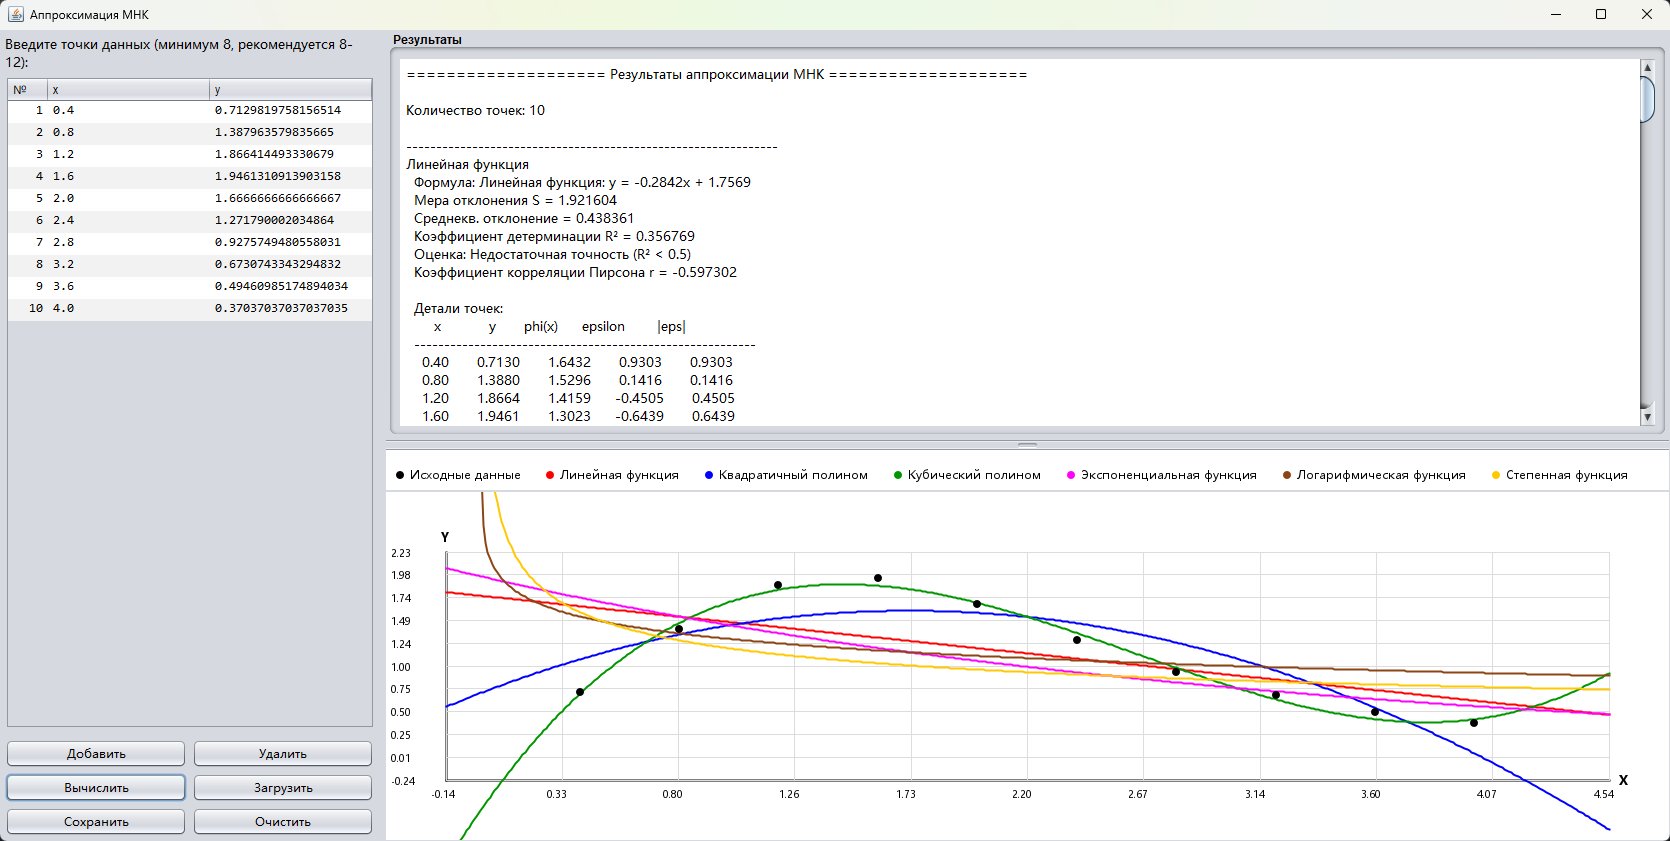
\includegraphics[width=1\linewidth]{pic/sp20260506_025543_709.png}
    \caption{Res 1}
    \label{fig:placeholder}
\end{figure}

\begin{figure}[H]
    \centering
    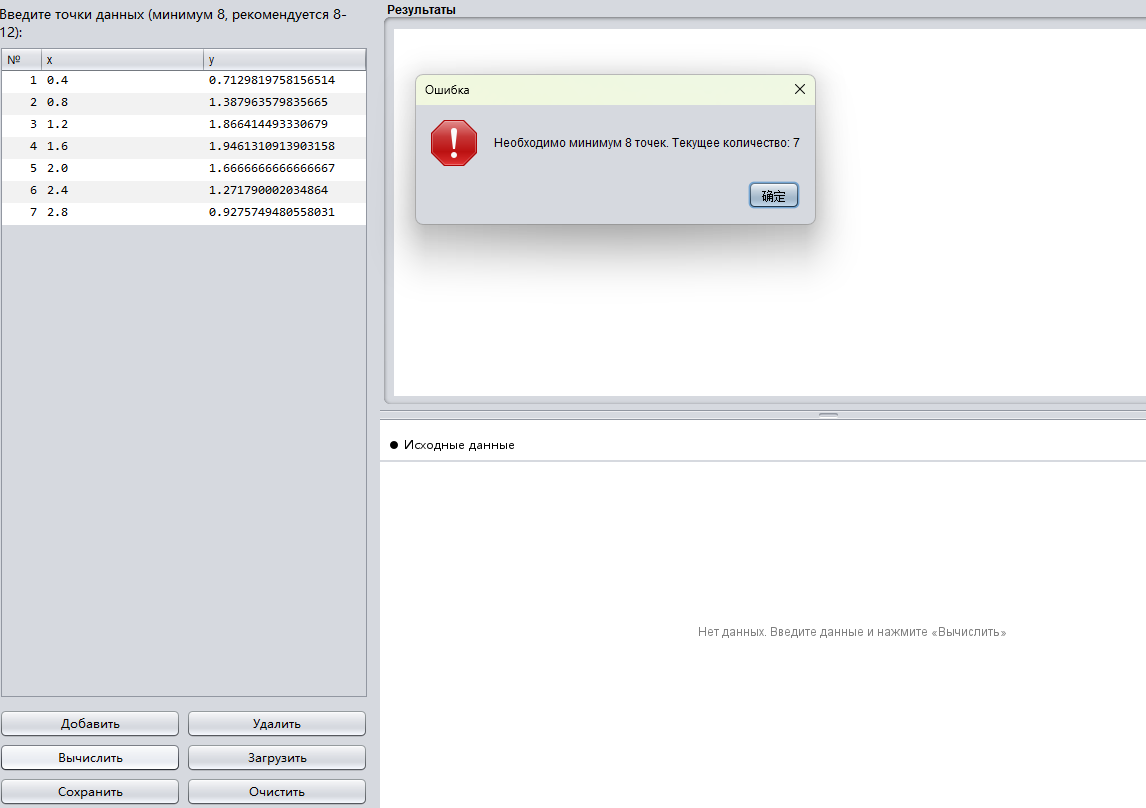
\includegraphics[width=1\linewidth]{pic/sp20260507_191317_271.png}
    \caption{Res 2}
    \label{fig:placeholder}
\end{figure}

\begin{figure}[H]
    \centering
    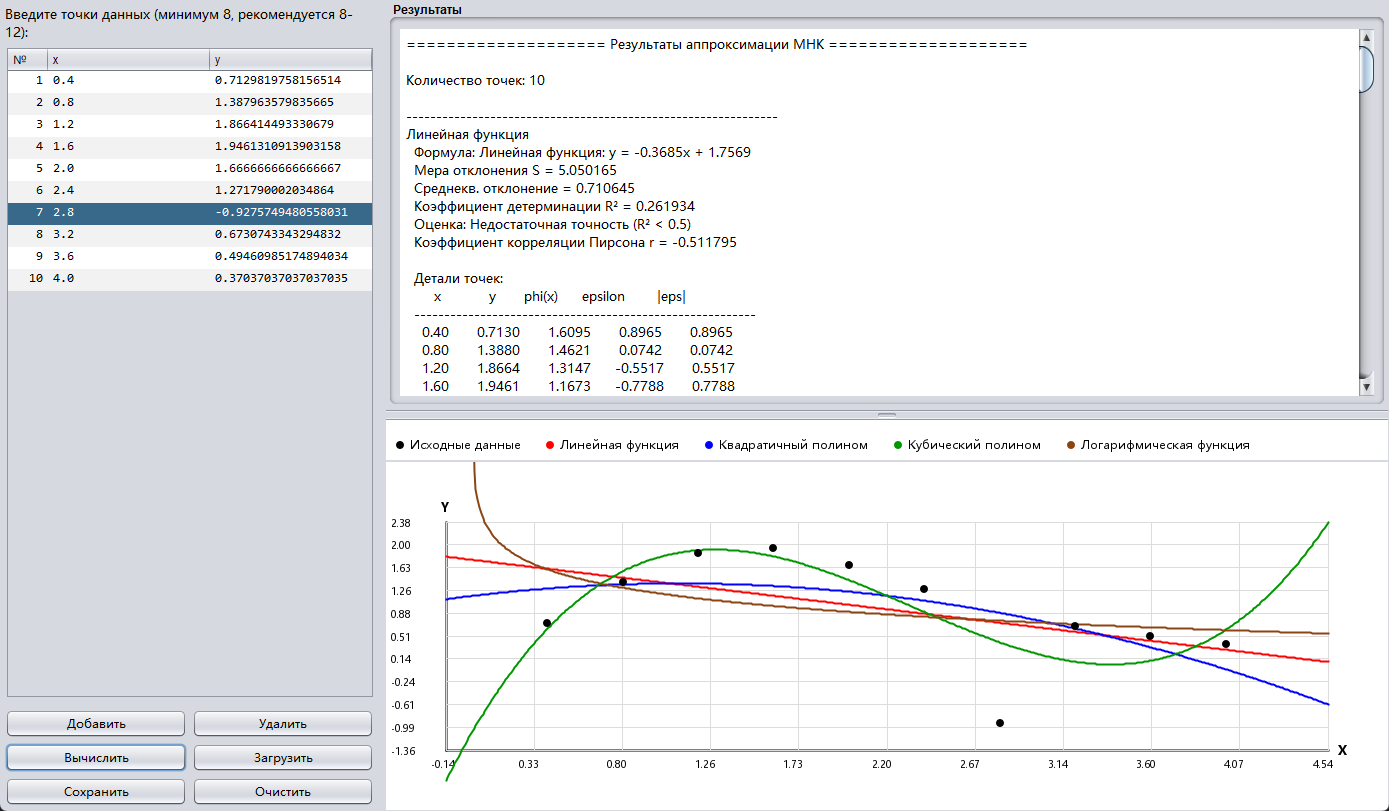
\includegraphics[width=1\linewidth]{pic/sp20260507_191414_887.png}
    \caption{Res 3}
    \label{fig:placeholder}
\end{figure}

\section{Вывод}

В программной части реализовано приложение на Java с графическим интерфейсом (Swing), поддерживающее шесть видов аппроксимирующих функций: линейную, квадратичную, кубическую, экспоненциальную, логарифмическую и степенную. Программа вычисляет коэффициенты МНК, меру отклонения $S$, \\среднеквадратичное отклонение $\delta$, коэффициент корреляции Пирсона (для линейной аппроксимации) и коэффициент детерминации $R^2$ с выводом соответствующей оценки. Результаты отображаются в табличном виде и на графиках.
